%% =====================================================================================
%% 5 In-game questions and scripted partners.
%% Numbers: tables/num_probes.tex (analysis/probes.py), tables/num_scripted.tex and
%% tables/tab_settled.tex (analysis/scripted.py). Figures: fig_knowdo.pdf, fig_scripted.pdf.
%% Wording rule: probe answers come from separate calls that never enter the game, so
%% the claim is a dissociation between answers and play, never that an answer "causes"
%% or "fails to cause" an action.
%% =====================================================================================
\section{Answers track the risk; play does not}
\label{sec:knowing}

A flat response to risk has a cheap explanation: perhaps the agents do not understand the
game. We test this in two ways. We ask the playing agent which choice pays more, and we seat
it with partners whose behaviour is fixed, so that the \emph{best response}, the play that
earns the most against them, can be computed exactly.

\subsection{Asking the agent}

In \CntGamesProbe{} games we question the first seat in rounds 1, 5 and 10, on the state it
has just decided on. Each question is a separate call, and its answer never enters the game.
Of the \ProbeQuestions{} questions, \ProbeRuleQuestions{} ask about the rules, such as the
target or the allowed amounts. Agents answer \ProbeRulePct\% of them correctly, but these
questions only ask for numbers printed in the prompt, so they show that agents read the
rules, not that they understand them. We therefore rest on one value question, asked
verbatim:
\begin{quote}\small
\emph{Compare two strategies for the whole game. (A) You contribute 2 in every one of the 10
rounds and the group reaches the target, so you finish with 20 for certain. (B) You
contribute 0 in every round and the group does not reach the target, so you keep 40 unless
the disaster strikes. Which gives the higher AVERAGE final cash? Answer 1 if A is higher, 2
if B is higher, 0 if they are exactly equal.}
\end{quote}
The correct answer is B below $\popt$, A above it, and equal at $\popt$. A second value
question could be read in two ways and is not used.

\begin{figure}[t]
\centering
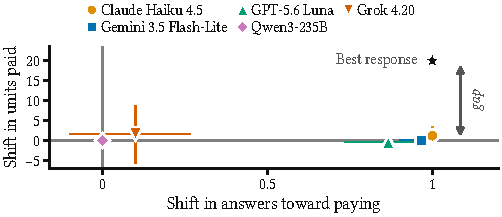
\includegraphics[width=\columnwidth]{figures/fig_knowdo.pdf}
\Description{A scatter plot with one point per model and 95 percent interval bars. The
horizontal axis is how far the model's answers move toward paying between catastrophe
probability 0.1 and 0.9; the vertical axis is how far its payment moves. Claude Haiku, Gemini
Flash-Lite and GPT Luna sit near 1 on the horizontal axis but near 0 on the vertical axis, far
below a star at 20 that marks the best response. Qwen sits at the origin and Grok close to
it.}
\caption{What agents say and do, from $p=0.1$ to $p=0.9$ in the same games (ten at each),
with 95\% intervals. Horizontal: drop in the share of answers saying that paying nothing pays
more on average; a correct answerer moves by 1. Vertical: change in what the questioned seat
pays. Star: a best responder beside fair-share partners.}
\label{fig:knowdo}
\end{figure}

\paragraph{Answers move with the risk; play does not.}
Claude Haiku and Gemini Flash-Lite answer the value question correctly almost every time, and GPT Luna in
\ProbeCorrectLunaPct\% of answers. All three change their answer with $p$
(Figure~\ref{fig:knowdo}, horizontal axis): in rounds 1 and 5 at $p=0.1$ they say that keeping pays more in
\ProbeThreeLowKeepPct\% of answers, and at $p=0.9$ they mostly say the opposite. Their
payments do not follow (Figure~\ref{fig:knowdo}, vertical axis): the same seats pay \ProbeThreeLowContrib{}
units at $p=0.1$ and \ProbeThreeHighContrib{} at $p=0.9$. Qwen and Grok do not show the
knowledge at all, with \ProbeCorrectQwenPct\% and \ProbeCorrectGrokPct\% correct. Qwen says
that keeping pays more in \ProbeQwenKeepPct\% of its answers at every risk level, and Grok
gives that answer in round 1 whatever the risk. The question lays out both strategies, which
is easier than finding the comparison inside the game, so the result is a gap between answers
and play, not evidence about what an agent computes when it decides.

\subsection{Playing against fixed partners}

Next we seat one model with five scripted partners of one kind: they always pay 0, always pay
2, always pay 4, or copy the group, starting at 2 and then paying the rounded average of the
other seats' previous round. The model is not told that its partners are scripted, but their
moves are in the history. We found the best response to each kind by trying all $3^{10}$
sequences of the model's own moves. Beside partners who always pay 0 the target cannot be
reached, and beside partners who always pay 4 it is reached without the model, so the best
response to both is to pay nothing. Paying becomes dominated, in the sense of
Section~\ref{sec:game}, only once the history settles the outcome.
Beside fair-share partners the best response is to pay nothing below
$\popt$ and exactly 20 above it; the copying partners never leave 2 and give the same
answer.

\paragraph{No model pays nothing where that is the best response.}
In none of the \ScrDominatedGames{} games beside these two kinds of partner does the model pay
nothing; the smallest total we see is \ScrMinTotalDominated{} units. Only \ScrOptimalGames{}
of \ScrGames{} games are exactly optimal, and \ScrOptimalAllTwenty{} one of them has a total
of 20, the fair share. The models land on the optimum only where the optimum is the default.

\paragraph{Partners matter; risk does not.}
We split the variation in what a model pays beside the three fixed-amount partners into parts
due to the partner, the risk and their interaction. For Claude Haiku, Gemini Flash-Lite, GPT Luna and Qwen, the
kind of partner explains \ScrOpponentShareMin\% to \ScrOpponentShareMax\% of the variation,
and the risk at most \ScrRiskShareMax\%. For an exact best responder in the same games, the
risk would explain \ScrBestResponderRiskShare\%. Beside fair-share partners, where the best
response jumps from 0 to 20 at $\popt$, no model's total differs by more than 2 units
between low and high risk. Grok's total follows neither the partner (\ScrGrokOpponentShare\%)
nor the risk (\ScrGrokRiskShare\%). Its game is decided by its first move, which it samples
before any history exists: it opens with 4 in \ScrGrokOpenFour{} of 200 games and mostly
repeats that opening, and this first move alone explains \ScrGrokFirstMoveShare\% of the
variation in its total.

\begin{figure}[t]
\centering
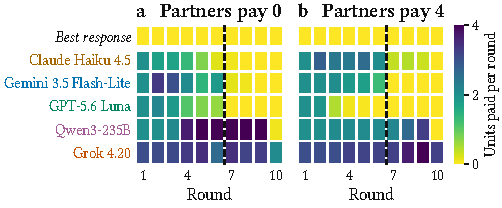
\includegraphics[width=\columnwidth]{figures/fig_scripted.pdf}
\Description{Two heatmaps with one row per model and one column per round, beside five
partners that always pay nothing and beside five that always pay four. Darker cells mean
larger payments. The top row, the best response, is light everywhere. GPT Luna's row turns
light within a few rounds and Gemini Flash-Lite and Claude Haiku turn light at a dashed line
after round six, while Qwen and Grok stay dark until round nine.}
\caption{One model beside five scripted partners, pooled over five risk levels (50 games per
row). A cell is the mean payment in one round; the top row is the best response, 0 in every
round. The dashed rule follows round 6, after which the outcome is settled in most games.}
\label{fig:scripted}
\end{figure}

\begin{table}[t]
\caption{Units a model pays per game before and after the outcome is settled, beside five
partners who always pay 0 or always pay 4 (50 games per entry). Given these partners, every
unit paid is wasted; units paid after settlement are wasted even for an agent that does not
know its partners are scripted.}
\label{tab:settled}
\small
% Generated by paper/AAMAS/analysis/scripted.py. Do not edit by hand.
\begin{tabular}{@{}lrrrr@{}}
\toprule
 & \multicolumn{2}{c}{Always 0} & \multicolumn{2}{c}{Always 4} \\
\cmidrule(lr){2-3}\cmidrule(l){4-5}
Model & Before & After & Before & After \\
\midrule
Claude Haiku 4.5 & 7.7 & 0.1 & 14.2 & 1.1 \\
Gemini 3.5 Flash-Lite & 13.6 & 0.2 & 10.9 & 0.0 \\
GPT-5.6 Luna & 8.5 & 0.0 & 4.5 & 0.0 \\
Qwen3-235B & 17.8 & 12.1 & 12.3 & 8.1 \\
Grok 4.20 & 19.6 & 11.1 & 16.7 & 16.2 \\
\bottomrule
\end{tabular}

\end{table}

\paragraph{Responses to partners take simple forms.}
The models respond to their partners, but not the way a best responder would
(Figure~\ref{fig:scripted}, Table~\ref{tab:settled}). Gemini Flash-Lite and Claude Haiku pay their usual
rate and then stop once the history shows that the outcome is settled. GPT Luna pays little even
before that point, above all beside partners who always pay 4, which is close to a best
response while it learns who its partners are. Qwen raises its payment to 4 beside partners
who pay nothing. Qwen and Grok keep paying large amounts after the outcome is settled, which
no belief about the partners can justify. Qwen's last-round rule also costs its partners:
beside five fair-share partners it pays 2 for nine rounds and then 0, and the table misses the
target in \ScrQwenFairMiss{} of 50 games, each time by exactly \ScrQwenFairShort{} units.
Gemini Flash-Lite in the same seat reaches the target in \ScrFlashFairReach{} of 50.
